\section*{Chapter 3: Design and Implementation}
\phantomsection \setcounter{section}{3} \setcounter{subsection}{0}
\addcontentsline{toc}{section}{\textit{Chapter 3: Design and Implementation}}

This chapter presents the design of the proposed LLM multi-agent negotiation framework for 5G network slice resource management and describes its implementation. Section~3.1 outlines the overall system architecture and the guiding design principles. Section~3.2 details the two-tier scheduling framework. Section~3.3 specifies the roles and internal logic of the individual agents. Section~3.4 defines the proposal--evaluation--negotiation protocol. Section~3.5 describes the Gymnasium-based simulation environment. Section~3.6 discusses the LangGraph-orchestrated workflow. Section~3.7 presents the baseline methods implemented for comparison.

\subsection{System Overview and Architectural Principles}

The proposed framework is organised into three loosely coupled layers, as illustrated in Figure~\ref{fig:sysarch}. The \emph{Agent Layer} defines the specialised agents and their configurations. The \emph{Collaboration Layer} implements inter-agent negotiation and conflict resolution. The \emph{Environment Layer} provides a standardised simulation interface that decouples the decision logic from the underlying simulator. The full system is orchestrated through LangGraph~\cite{langchain2024langgraph}, with a commercial LLM API (GPT-4 series) serving as the reasoning backbone.

\begin{figure}[h]
    \centering
    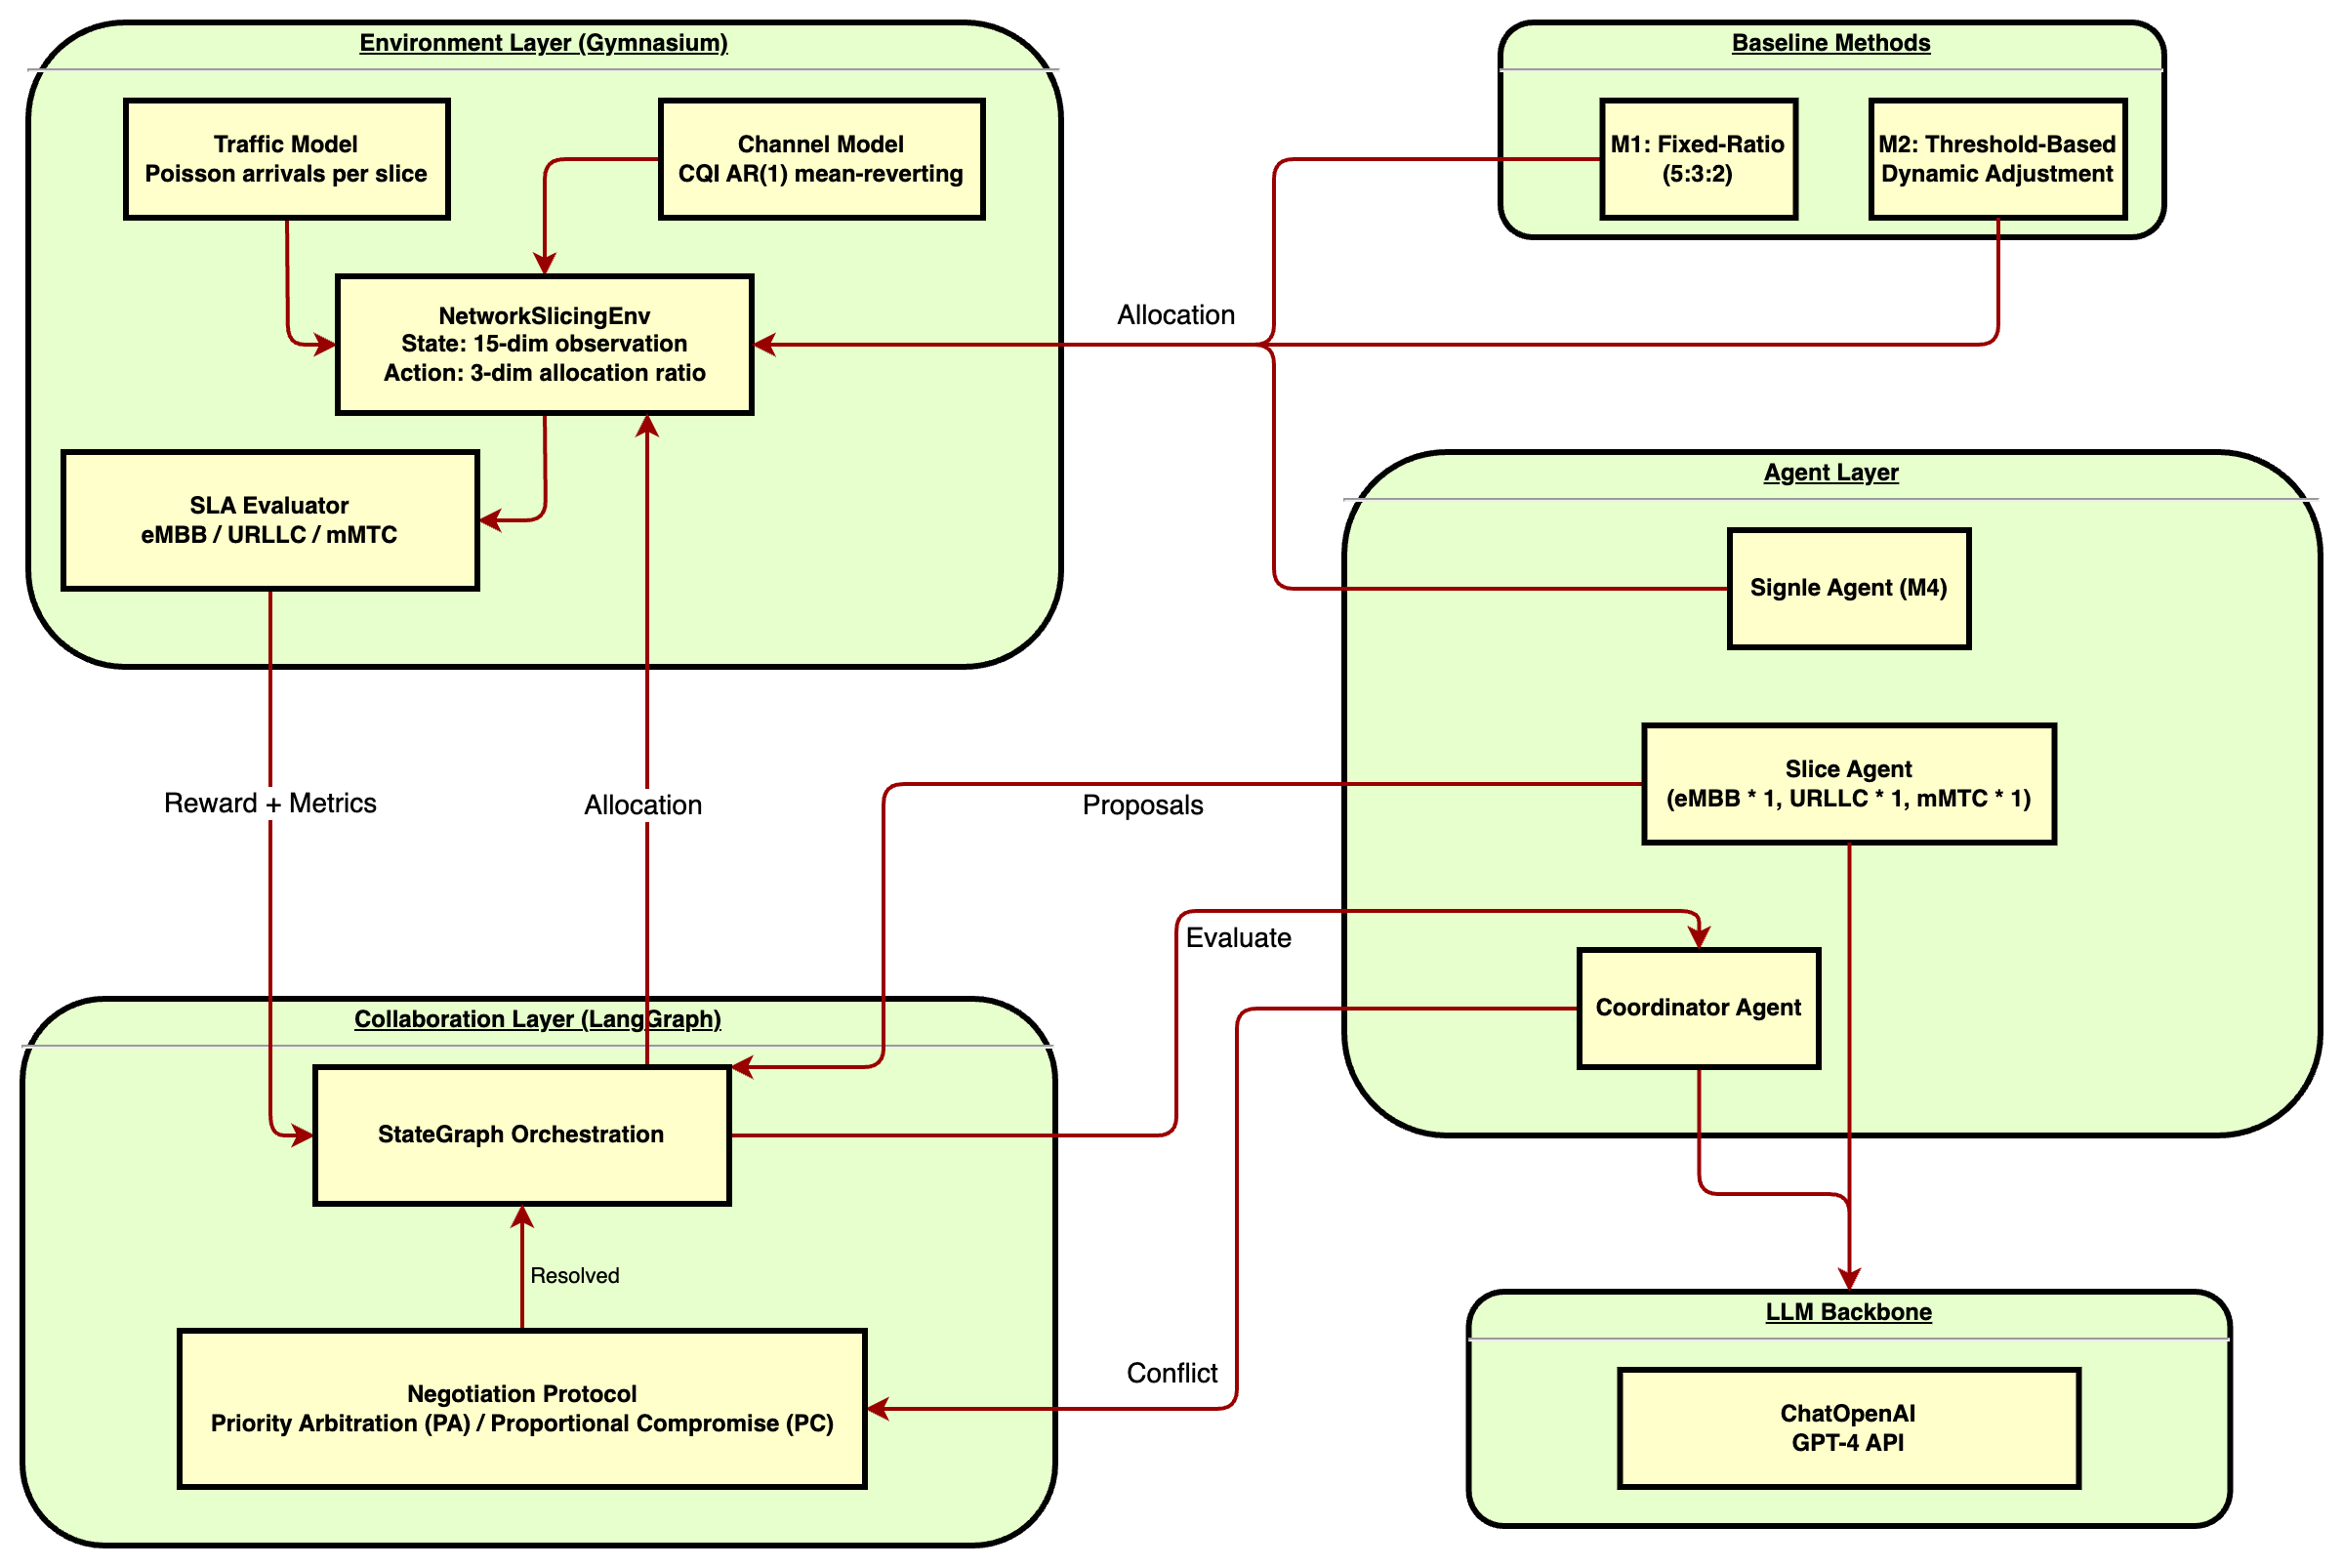
\includegraphics[width=0.95\textwidth]{figures/System Architecture.drawio.png}
    \caption{Overall system architecture of the proposed two-tier multi-agent framework.}
    \label{fig:sysarch}
\end{figure}

The design is guided by four principles:

\begin{itemize}
    \item \emph{Separation of timescales}: Slow semantic reasoning by LLM agents is decoupled from fast rule-based execution so that LLM inference latency does not propagate into the per-TTI control loop.
    \item \emph{Role specialisation}: Each slice type is represented by a dedicated agent whose prompts and internal reasoning are tailored to the characteristics of that slice, while a global coordinator agent is responsible exclusively for cross-slice arbitration.
    \item \emph{Structured communication}: Inter-agent messages are exchanged as structured JSON artefacts rather than as free-form natural language, in the spirit of MetaGPT~\cite{hong2023metagpt}, in order to reduce information loss and to make the behaviour of the system inspectable.
    \item \emph{Graceful degradation}: Whenever the LLM layer fails to produce a decision within a predefined latency budget, the system automatically falls back to a rule-based controller, so that the operational stability of the network is never contingent on the responsiveness of an external API.
\end{itemize}

\subsection{Two-Tier Scheduling Framework}

A central challenge addressed by the design is the order-of-magnitude gap between the inference latency of contemporary LLMs --- typically hundreds of milliseconds to a few seconds per call --- and the millisecond-level timescale at which radio scheduling decisions must be taken. Placing an LLM directly on the per-TTI control loop is therefore infeasible. The proposed framework adopts an explicit two-tier scheduling architecture, illustrated in Figure~\ref{fig:twotier}.

\begin{figure}[h]
    \centering
    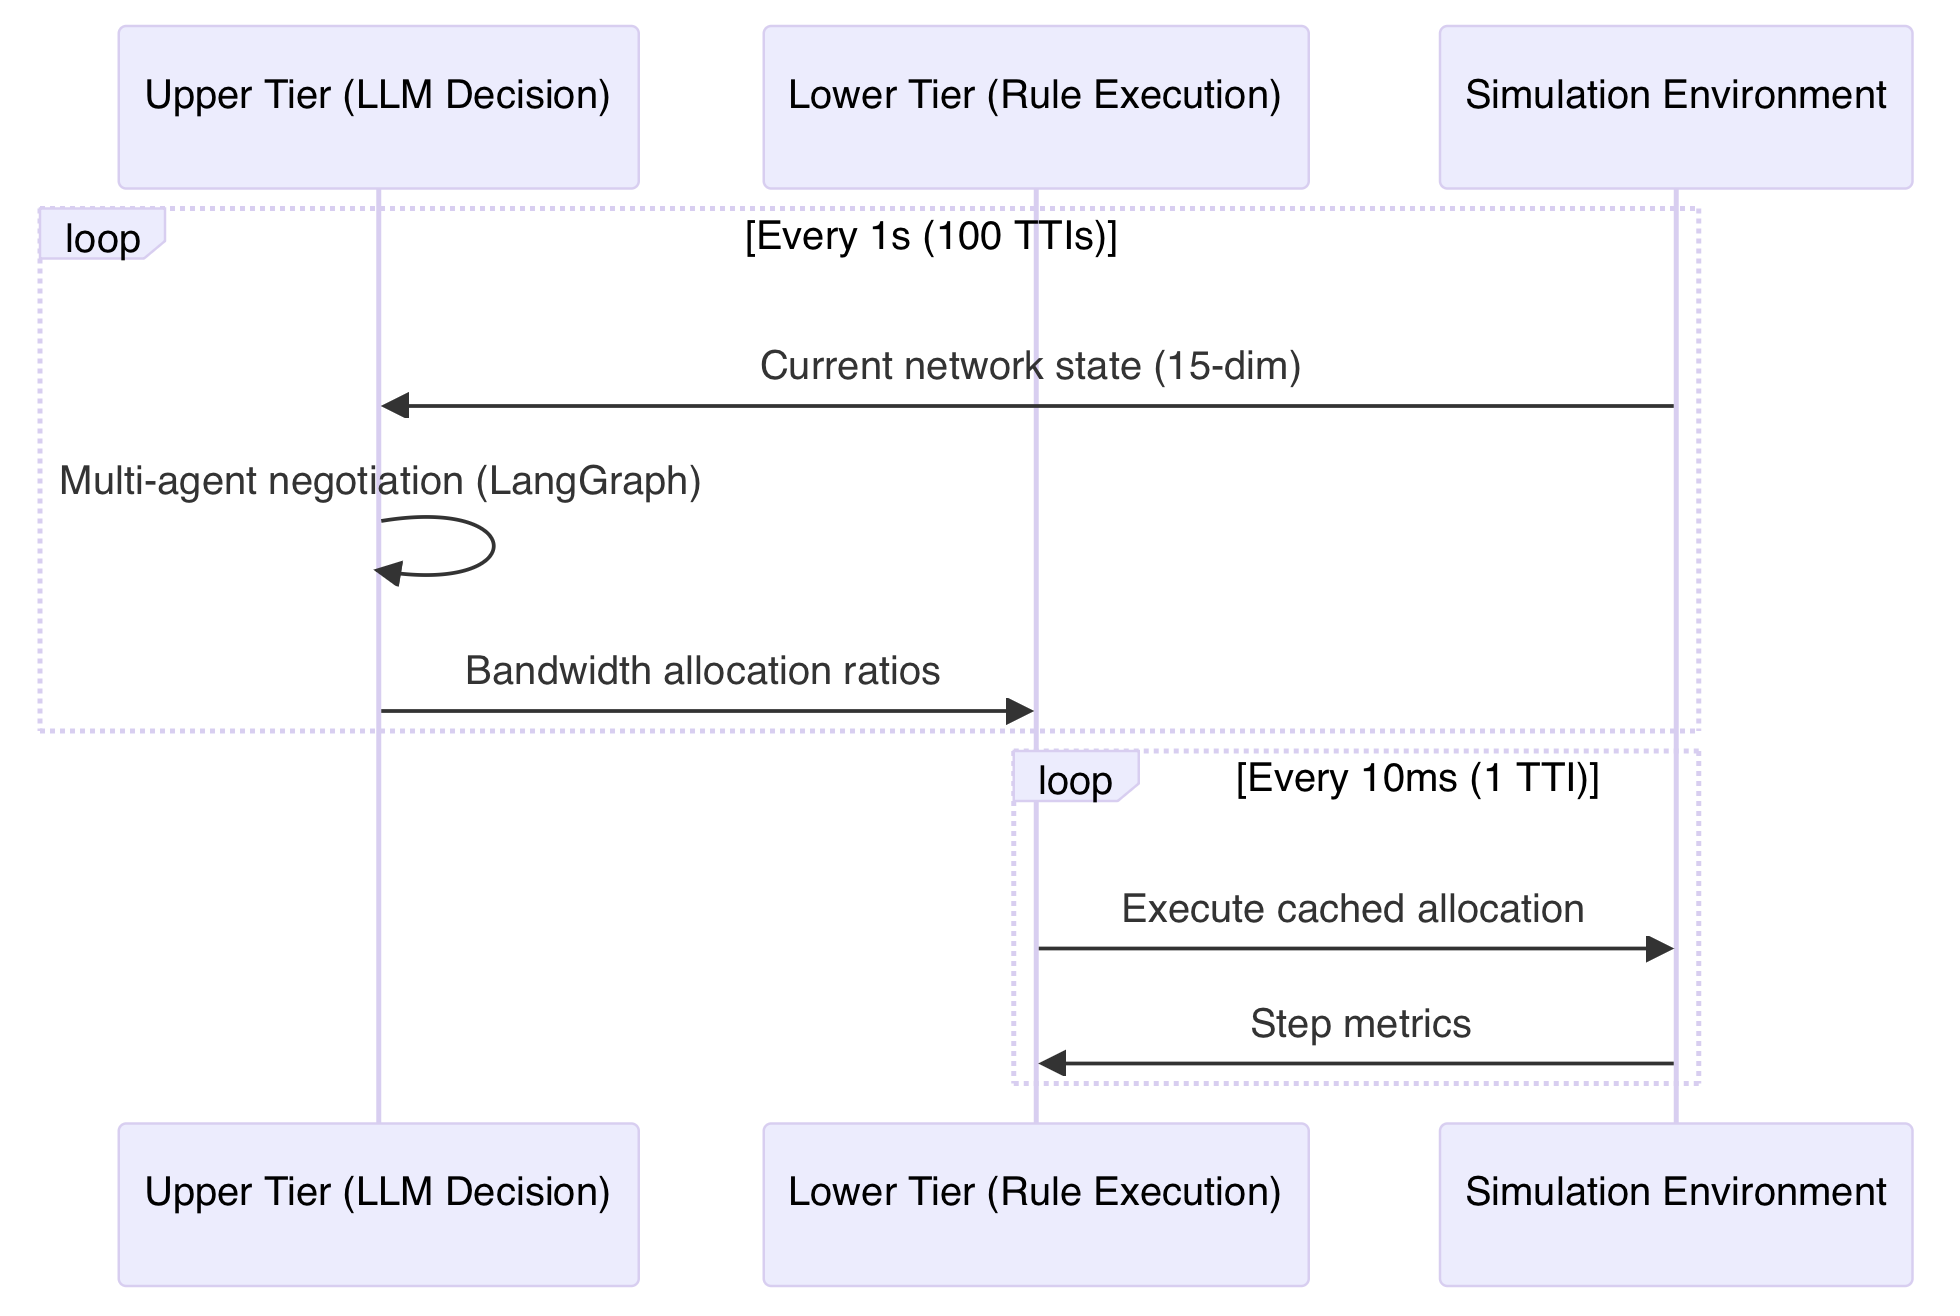
\includegraphics[width=0.9\textwidth]{figures/Two-Tier Scheduling.png}
    \caption{Two-tier scheduling: slow LLM policy updates at the upper tier and fast rule-based execution at the lower tier.}
    \label{fig:twotier}
\end{figure}

The \emph{upper tier}, or LLM decision layer, is triggered once every 100~TTIs (approximately one second) in the baseline configuration. At each trigger, the slice-manager agents and the global coordinator agent execute one round of the proposal--evaluation--negotiation protocol described in Section~3.4 and update the inter-slice bandwidth allocation quotas. An emergency decision can additionally be triggered when the measured SLA violation rate exceeds a predefined threshold, allowing the framework to react to sudden changes in traffic conditions.

The \emph{lower tier}, or fast execution layer, operates at a TTI-level granularity of approximately 10\,ms. Within each decision window, it executes a cached rule-based strategy that enforces the inter-slice quotas produced by the upper tier, without invoking the LLM. This layer is responsible for per-user scheduling inside each slice and for monitoring SLA-related indicators that feed back into the upper tier.

A \emph{maximum decision latency threshold} of 2~seconds is enforced on the upper tier. If the LLM layer fails to return a decision within this budget, the system automatically falls back to the most recent valid allocation or, in the absence of one, to a default fixed-ratio policy (eMBB\,:\,URLLC\,:\,mMTC $= 0.5 : 0.3 : 0.2$). This fallback behaviour is a direct consequence of the graceful degradation principle introduced in Section~3.1.

\subsection{Agent Role Definition and Internal Logic}

The proposed framework defines four agents: one slice-manager agent per slice type (eMBB, URLLC, mMTC) and a single global coordinator agent. Each agent shares a common internal structure consisting of three modules --- \emph{Perception}, \emph{Planning} and \emph{Action} --- in line with the cognitive architecture pattern adopted by WirelessAgent~\cite{tong2025wirelessagent} and surveyed more broadly by Wang \emph{et al.}~\cite{wang2023agentsurvey}.

\paragraph{Slice Manager Agent.} A slice-manager agent is instantiated for each of the three slice types. The Perception module converts the numerical state of the slice --- user count, average Channel Quality Indicator (CQI), buffer occupancy and current SLA satisfaction rate --- into a structured natural-language description that is fed into the LLM prompt. The Planning module uses Chain-of-Thought prompting~\cite{wei2022cot} to assess the current resource demand of the slice in light of its SLA targets. The Action module outputs a resource demand proposal as a structured JSON object containing four fields:

\begin{itemize}
    \item \texttt{requested}: the desired bandwidth fraction;
    \item \texttt{minimum}: the minimum acceptable fraction (always $\geq 0.05$);
    \item \texttt{priority}: a declaration of ``high'', ``medium'' or ``low'';
    \item \texttt{justification}: a brief natural-language rationale.
\end{itemize}

Each agent carries a role-specific system prompt that encodes the SLA requirements and operational characteristics of its assigned slice. When the coordinator provides feedback after a failed compatibility check, the slice agent can generate a revised \emph{counter-proposal} that takes the feedback into account while still advocating for its slice's interests.

\paragraph{Global Coordinator Agent.} A single global coordinator agent is responsible for cross-slice arbitration. Its Perception module aggregates the proposals produced by the slice-manager agents together with the global resource state. The Planning module determines whether the proposals are jointly compatible --- that is, whether the sum of the requested shares can be satisfied within the available bandwidth budget. If the proposals are compatible, they are approved directly. If a conflict is detected, the coordinator outputs a structured evaluation as a JSON object containing:

\begin{itemize}
    \item \texttt{compatible}: a boolean indicating whether proposals are jointly feasible;
    \item \texttt{allocation}: a dictionary mapping each slice name to its allocated fraction;
    \item \texttt{feedback}: a natural-language rationale or per-slice suggestions.
\end{itemize}

The priority order URLLC $>$ eMBB $>$ mMTC is encoded in the coordinator's system prompt. The allocation produced by the coordinator is always renormalised to sum to~1, with each slice receiving at least 0.05.

\subsection{Proposal--Evaluation--Negotiation Protocol}

When the coordinator detects that the aggregate demand exceeds the available capacity, a three-phase negotiation protocol is triggered. The overall message flow is shown in Figure~\ref{fig:negflow}.

\begin{figure}[h]
    \centering
    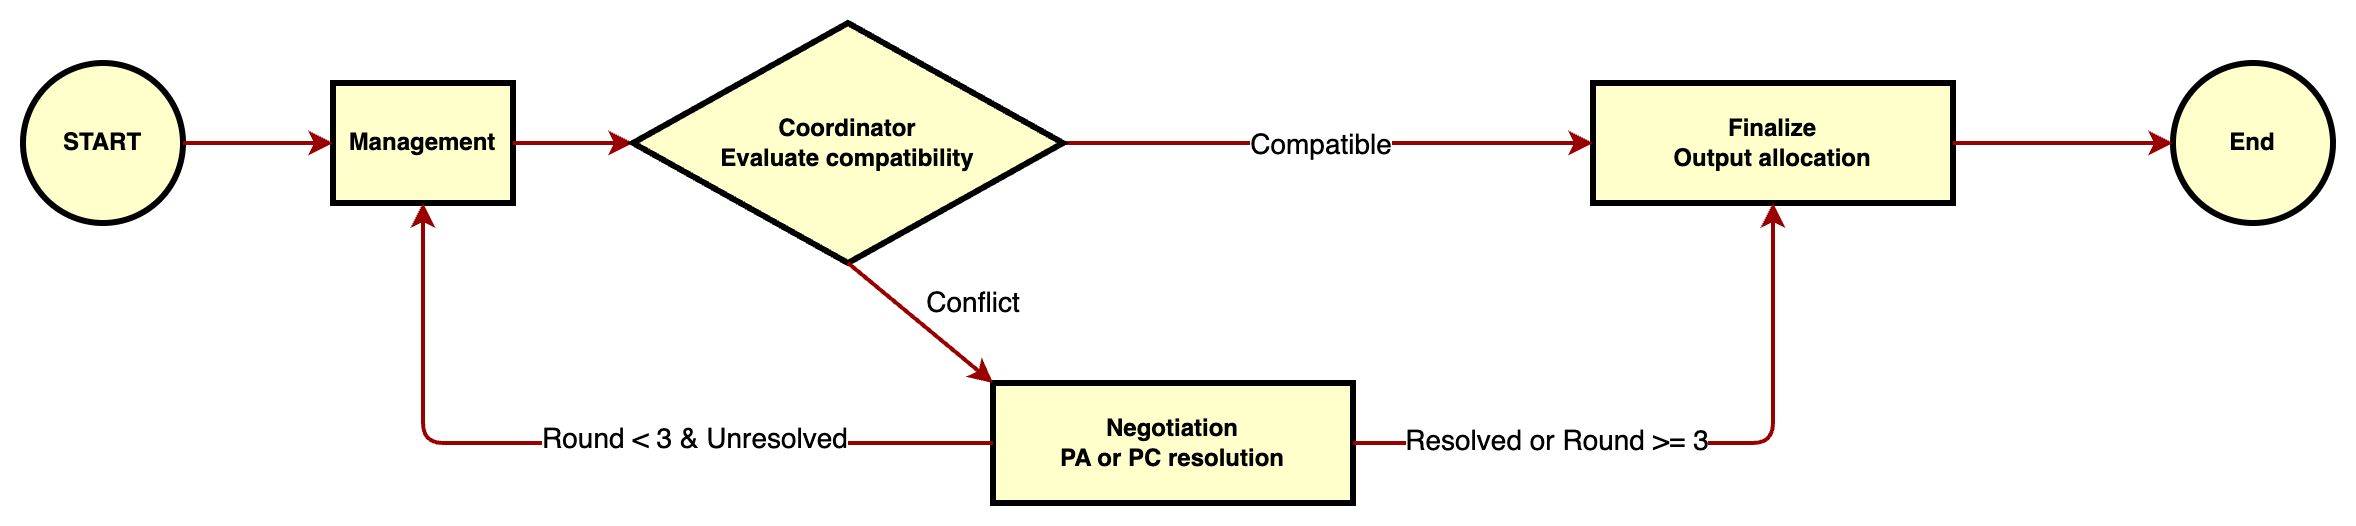
\includegraphics[width=0.95\textwidth]{figures/Multi-Agent Negotiation Flow.drawio.png}
    \caption{Message flow of the three-phase proposal--evaluation--negotiation protocol.}
    \label{fig:negflow}
\end{figure}

\paragraph{Phase~1 --- Proposal.} Each slice-manager agent independently evaluates its current demand and submits a resource proposal as a structured JSON message containing its requested share, minimum acceptable share, priority declaration and justification.

\paragraph{Phase~2 --- Evaluation.} The global coordinator agent evaluates the joint feasibility of the proposals. Feasibility checks include whether the total requested bandwidth exceeds unity and whether hard priority rules are satisfied (e.g., URLLC requirements take precedence).

\paragraph{Phase~3 --- Negotiation.} If a conflict is detected, a deterministic resolution protocol is invoked. The implementation provides two strategies:

\begin{itemize}
    \item \textbf{Priority Arbitration (PA):} Each slice receives its minimum allocation of 0.05. The remaining capacity is distributed in priority order (URLLC $>$ eMBB $>$ mMTC), with each slice receiving up to its requested share before the next slice is considered.

    \item \textbf{Proportional Compromise (PC):} Each slice is first guaranteed its declared minimum. The residual capacity ($1.0 - \sum \text{minimums}$) is then distributed in proportion to the excess demand ($\text{requested} - \text{minimum}$) of each slice.
\end{itemize}

After a resolution round, the graph may loop back to the slice-agent node for a further round of counter-proposals, up to a maximum of 3 negotiation rounds. If the maximum is reached without the coordinator declaring compatibility, the most recent resolution is accepted as the final allocation. This bounded iteration controls both latency and token cost.

\subsection{Gymnasium-Based Simulation Environment}

A custom 5G network slicing simulation environment is built using the Gymnasium framework~\cite{brockman2016gym}. The environment models the dynamics of user arrivals, channel quality variations, buffer accumulation and SLA evaluation at each decision step. All parameters are listed in Table~\ref{table:envparams}.

\begin{table}[h]
  \centering
  \begin{spacing}{1.35}
  \caption{Key parameters of the simulation environment.}\vspace{0.7em}
  \label{table:envparams}
    \begin{tabular}{|p{4.5cm}|p{5cm}|p{4cm}|}
    \hline
    \textbf{Parameter} & \textbf{Value} & \textbf{Notes} \\
    \hline
    System bandwidth & 100 MHz & Reference NR n78 band \\
    \hline
    Slice types & eMBB, URLLC, mMTC & 3GPP canonical types \\
    \hline
    Maximum users & 100 & Per decision cycle \\
    \hline
    Poisson arrival rates & [50, 30, 20] & eMBB, URLLC, mMTC \\
    \hline
    CQI means & [9, 10, 7] & eMBB, URLLC, mMTC \\
    \hline
    CQI reversion rate ($\alpha$) & 0.15 & AR(1) mean reversion \\
    \hline
    CQI noise std ($\sigma$) & 1.2 & Gaussian \\
    \hline
    Minimum allocation & 0.05 & Per slice \\
    \hline
    Burst onset cycle & 50 & eMBB $\lambda$ doubles \\
    \hline
    Burst multiplier & 2.0 & eMBB arrival rate \\
    \hline
    SLA sliding window & 10 steps & For satisfaction rate \\
    \hline
    Decision cycles per episode & 100 & \texttt{max\_steps} \\
    \hline
    \end{tabular}
  \end{spacing}
\end{table}

\subsubsection{State Space}

The observation space comprises 15 continuous dimensions, each normalised to $[0,1]$, as defined in Table~\ref{table:statespace}.

\begin{table}[h]
  \centering
  \begin{spacing}{1.35}
  \caption{State space definition and normalisation.}\vspace{0.7em}
  \label{table:statespace}
    \begin{tabular}{|p{2.5cm}|p{5.5cm}|p{2.5cm}|p{3cm}|}
    \hline
    \textbf{Dimension} & \textbf{Meaning} & \textbf{Range} & \textbf{Normalisation} \\
    \hline
    $n_i$ ($\times 3$) & Current user count per slice & $[0, N_{\max}]$ & $/\, N_{\max}$ \\
    \hline
    $\bar{c}_i$ ($\times 3$) & Average CQI per slice & $[1, 15]$ & $/\, 15$ \\
    \hline
    $b_i$ ($\times 3$) & Buffer occupancy per slice & $[0, 1]$ & Raw value \\
    \hline
    $a_i$ ($\times 3$) & Current bandwidth allocation & $[0, 1]$ & Raw value \\
    \hline
    $s_i$ ($\times 3$) & SLA satisfaction rate (sliding window) & $[0, 1]$ & Raw value \\
    \hline
    \end{tabular}
  \end{spacing}
\end{table}

\subsubsection{Action Space}

The action space is a continuous 3-dimensional vector $\mathbf{a} = (a_{\text{eMBB}},\, a_{\text{URLLC}},\, a_{\text{mMTC}})$ subject to $\sum_i a_i = 1$ and $a_i \geq 0.05$. Raw actions are clipped to $[0,1]$, the minimum allocation constraint is enforced, and the result is renormalised to ensure the fractions sum to unity.

\subsubsection{Channel and Throughput Model}

Channel quality is modelled using a discrete Ornstein--Uhlenbeck (AR(1)) process for each slice:
\begin{equation}
    \text{CQI}_i(t+1) = \text{CQI}_i(t) + \alpha\bigl(\mu_i - \text{CQI}_i(t)\bigr) + \sigma\,\varepsilon_t, \quad \varepsilon_t \sim \mathcal{N}(0,1)
    \label{eq:cqi}
\end{equation}
where $\mu_i$ is the long-term mean CQI for slice $i$, $\alpha$ is the reversion rate and $\sigma$ is the noise standard deviation. CQI values are rounded to integers and clipped to $[1, 15]$. Spectral efficiency is obtained from the standard 3GPP CQI-to-spectral-efficiency mapping table. User-level throughput is computed as:
\begin{equation}
    T_{i,\text{user}} = \frac{a_i \cdot B_{\text{total}} \cdot \text{SE}(\text{CQI}_i) \cdot M}{n_i}
    \label{eq:throughput}
\end{equation}
where $B_{\text{total}} = 100$\,MHz is the total bandwidth, $\text{SE}(\cdot)$ is the spectral efficiency function, $M = 20$ is a MIMO and coding gain multiplier, and $n_i$ is the number of users in slice~$i$.

\subsubsection{SLA Definitions}

The SLA metrics used in this simulation represent relative priority isolation rather than strict 3GPP end-to-end physical-layer metrics. Table~\ref{table:sla} defines the three SLA conditions.

\begin{table}[h]
  \centering
  \begin{spacing}{1.35}
  \caption{Simulation-layer SLA approximations and design intent.}\vspace{0.7em}
  \label{table:sla}
    \begin{tabular}{|p{1.8cm}|p{5.5cm}|p{3.5cm}|p{2.5cm}|}
    \hline
    \textbf{Slice} & \textbf{SLA Condition} & \textbf{Design Intent} & \textbf{Application} \\
    \hline
    eMBB & Average user throughput $\geq 50$\,Mbps & High throughput guarantee & Video streaming \\
    \hline
    URLLC & 99th-percentile queuing delay $\leq 10\%$ of eMBB delay & Relative priority guarantee & Industrial control \\
    \hline
    mMTC & Access success rate $\geq 95\%$ & Massive access guarantee & IoT sensors \\
    \hline
    \end{tabular}
  \end{spacing}
\end{table}

For URLLC, the 99th-percentile delay is approximated as 2.3 times the mean queuing delay (based on an exponential service model), and the delay is computed as a packet-weight-to-capacity ratio. The mMTC access rate is modelled as the ratio of allocated capacity to the number of requesting devices.

\subsubsection{Reward Function}

The reward at each step is a weighted combination of three normalised terms:
\begin{equation}
    R = w_S \cdot \bar{S} + w_U \cdot U - w_V \cdot V
    \label{eq:reward}
\end{equation}
where $\bar{S}$ is the mean SLA satisfaction rate across slices (computed over a sliding window of 10 steps), $U$ is the bandwidth utilisation, and $V = 1 - \bar{S}_{\text{instant}}$ is the instantaneous violation penalty. The default weights are $w_S = 0.5$, $w_U = 0.3$ and $w_V = 0.2$.

\subsubsection{Traffic Scenarios}

Two traffic scenarios are used throughout the experiments:
\begin{itemize}
    \item \textbf{Steady-state:} User arrival rates follow Poisson processes with fixed means (eMBB: 50, URLLC: 30, mMTC: 20) throughout the episode.
    \item \textbf{Burst:} Identical to steady-state for the first 49 decision cycles; from cycle 50 onward, the eMBB arrival rate is doubled ($\lambda_{\text{eMBB}} = 100$), simulating a sudden surge in mobile broadband demand.
\end{itemize}

\subsection{LangGraph-Orchestrated Agent Workflow}

The multi-agent decision process is orchestrated using LangGraph~\cite{langchain2024langgraph}, a state-machine library that represents the agent workflow as a directed graph with typed state transitions. The graph carries a shared state object (\texttt{MASState}) through four node types:

\begin{enumerate}
    \item \textbf{Slice Agents node:} Invokes all three slice-manager agents in sequence, each producing a proposal (or counter-proposal if feedback is available from a prior round).
    \item \textbf{Coordinator node:} Invokes the coordinator agent to evaluate the joint feasibility of the proposals and produce an allocation.
    \item \textbf{Negotiation node:} If the coordinator declares the proposals incompatible, a deterministic resolution function (PA or PC) computes an allocation from the proposals.
    \item \textbf{Finalize node:} Extracts the final allocation from either the coordinator's approved allocation or the negotiation resolution.
\end{enumerate}

Conditional edges connect the coordinator node to either the finalize node (if proposals are compatible) or the negotiation node (if a conflict is detected). After negotiation, the graph may loop back to the slice-agents node for another round, up to the configured maximum of 3~rounds.

The no-negotiation variant (M5-NoNeg) uses a simplified graph in which the coordinator node connects directly to the finalize node, with no negotiation or loopback edges. In this variant, the coordinator's single-round allocation is used as the final decision.

\subsection{Baseline Methods and Implementation Details}

Six methods are implemented and compared, as summarised in Table~\ref{table:methods}.

\begin{table}[h]
  \centering
  \begin{spacing}{1.35}
  \caption{Summary of compared methods (M1--M5 and variants).}\vspace{0.7em}
  \label{table:methods}
    \begin{tabular}{|p{1.5cm}|p{2.8cm}|p{3cm}|p{6cm}|}
    \hline
    \textbf{ID} & \textbf{Method} & \textbf{Category} & \textbf{Description} \\
    \hline
    M1 & Fixed-Ratio & Rule-based & Static allocation (eMBB\,:\,URLLC\,:\,mMTC $= 0.5 : 0.3 : 0.2$) \\
    \hline
    M2 & Threshold-based & Rule-based & Dynamic adjustment triggered when any slice's SLA satisfaction rate drops below 0.8; bandwidth is transferred from the best-performing slice \\
    \hline
    M3 & PPO & Deep RL & MLP policy network trained with Proximal Policy Optimisation~\cite{schulman2017ppo} using Stable-Baselines3~\cite{raffin2021sb3} \\
    \hline
    M4 & Single-Agent LLM & Single-agent LLM & One GPT-4 agent with CoT reasoning; no multi-agent collaboration \\
    \hline
    M5-PA & Multi-Agent (PA) & Multi-agent LLM & Slice agents + coordinator + Priority Arbitration negotiation \\
    \hline
    M5-PC & Multi-Agent (PC) & Multi-agent LLM & Slice agents + coordinator + Proportional Compromise negotiation \\
    \hline
    \end{tabular}
  \end{spacing}
\end{table}

\paragraph{Rule-Based Baselines (M1, M2).} M1 applies a fixed allocation ratio throughout the episode, following commonly adopted traffic composition settings~\cite{nasser2025hybrid}. M2 monitors the sliding-window SLA satisfaction rate for each slice; when any slice falls below a threshold of 0.8, it transfers a small amount of bandwidth (0.05) from the slice with the highest current SLA rate, subject to the minimum allocation constraint.

\paragraph{DRL Baseline (M3).} The PPO agent~\cite{schulman2017ppo} is implemented using Stable-Baselines3~\cite{raffin2021sb3} with an MLP policy network. Training uses a mixed-scenario wrapper that randomly selects between steady-state and burst scenarios at each episode reset (burst probability 0.4). Training hyperparameters include learning rate $3 \times 10^{-4}$, 1024 steps per update, batch size 64, 10 epochs per update, and discount factor $\gamma = 0.99$. Early stopping is applied when the mean reward change over the most recent 100~episodes falls below 0.5\%, with a maximum of 2000~training episodes.

\paragraph{Single-Agent LLM Baseline (M4).} A single GPT-4 agent receives the full environment state as a natural-language description and outputs a 3-dimensional allocation vector via Chain-of-Thought reasoning. No inter-agent collaboration or negotiation takes place.

\paragraph{Multi-Agent LLM (M5).} The full multi-agent framework described in Sections~3.1--3.6, tested with both PA and PC negotiation strategies. The no-negotiation ablation (M5-NoNeg) retains the three slice agents and the coordinator but removes the negotiation loop, so that the coordinator's initial allocation is used directly.

%% ======== TEMPLATE GUIDANCE (retained per instructions) ========
% Normally there will be a part about the design and implementation of the system, especially for an implementation type of project. However, every project has its unique phases so you should talk to your supervisor about it.
